
\chapter{Use Cases} \label{use_cases}

The main purpose of the current chapter is to demonstrate the functionalities of the web platform, by building reproducible analysis pipelines using real data from previously published studies in the host group, while trying to show how to perform most of the available analyses in the web platform. For this purpose, two distinct datasets were used. The first use case is the discrimination of propolis samples from southern Brazil according to their chemical profile (using \gls{uv} data) \citep{tomazzoli2015discrimination}, while the second use case consists in the chemical and enzymatic composition screening in several genotypes of cassava roots during \gls{ppd} (using \gls{ir} data) \citep{uarrota2014metabolomics}.


\section{Propolis}

\subsection{Context}

The propolis resinous substance is collected by honeybees \textit{Apis mellifera} from various plant sources and added to salivary enzymes, beeswax, and pollen. They use it to seal openings and for protection against microorganisms and insects.

However, this substance also offers a broad spectrum of biological activities, including, for instance, cytotoxic, anti-herpes, free radical scavenging, antimicrobial, and anti-HIV activities, being used in both cosmetic and pharmaceutical markets. Therefore, the botanical origin of propolis is extremely important to guarantee that raw materials of superior quality are supplied to those markets.

Since the quality of the propolis depends, among other variables, on the local flora,
which is strongly influenced by (a)biotic factors over the seasons, the main scope of the study was to determine the harvest season effect on the chemical profile of this substance.

For this purpose, propolis samples from \textit{A. mellifera} were collected in Southern Brazil throughout 2014, and samples visually classified according to their color. The \gls{uv} absorbance values were recorded using a spectral window of 280-800 $\eta m$ \citep{tomazzoli2015discrimination}.


\subsection{Data Loading} \label{propolis_loading}

Assuming the user has already created a project with both data and metadata files, the dataset can be easily created through the \textit{Choose Files} button on the header. This step is done by directly importing a project from the user's stored projects and setting the file specifications to create the dataset, as observed in \autoref{propolis_import_project}.

\begin{figure}[h]
	\centering
	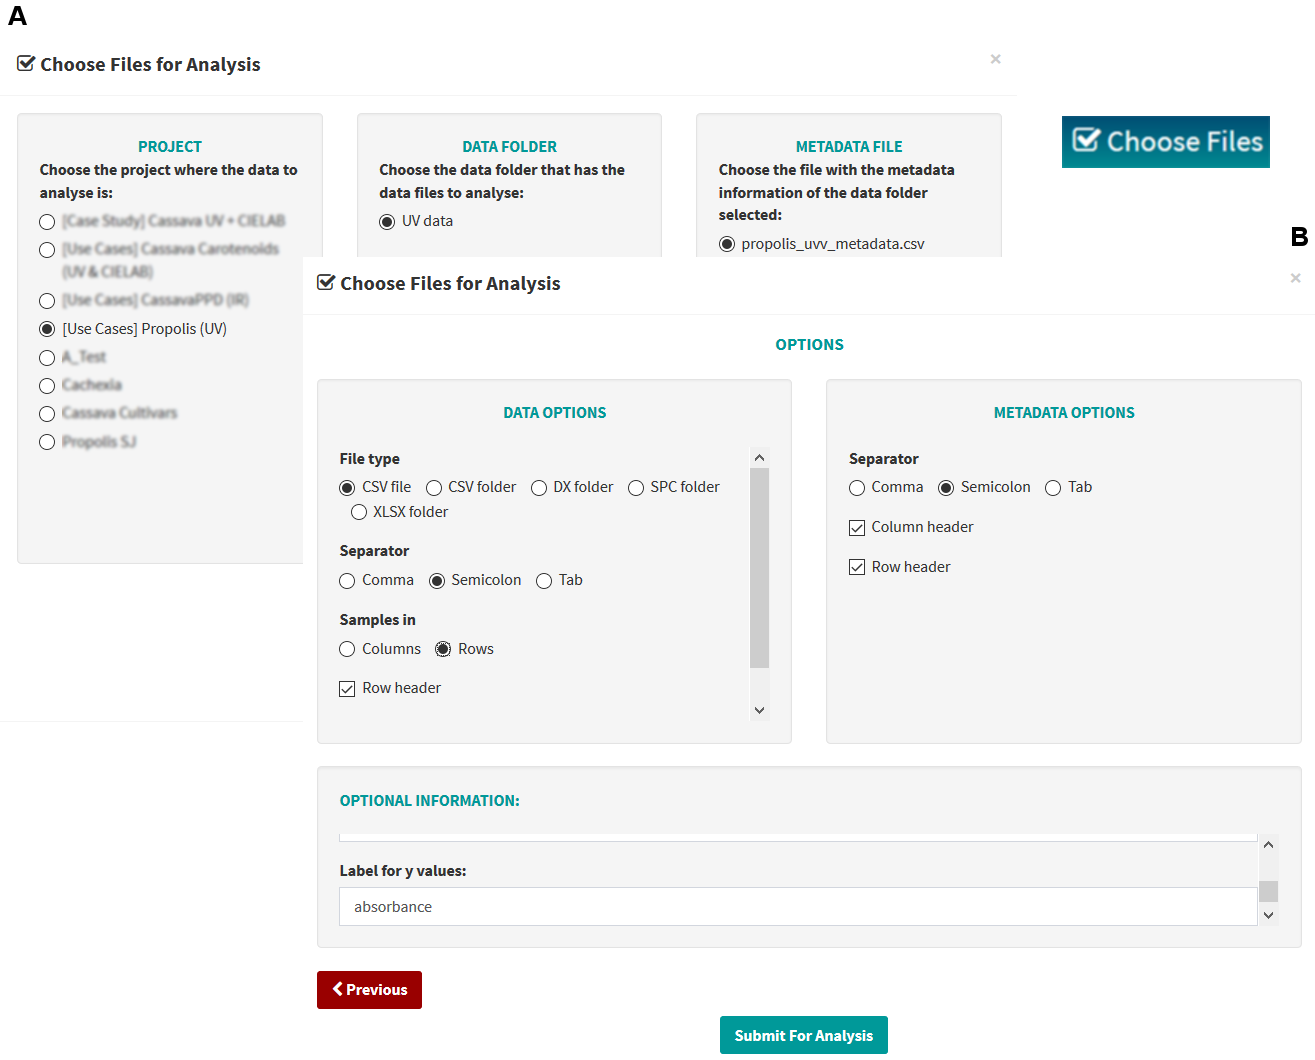
\includegraphics[width=1\linewidth]{Imagens/Propolis/import_project}
	\caption{Creating the propolis dataset for analysis. Upon clicking the \textit{Choose Files} button on the header, a window appears with all user's projects and respective folders/files (\textbf{A}). After selecting the desired project, the file specifications must be chosen to create the dataset (\textbf{B}).}
	\label{propolis_import_project}
\end{figure}


\subsection{Data Overview}

Once the dataset is created, its information can be easily accessed in the \textit{Data Visualization} page. 
In \autoref{propolis_data_overview}, the summary of the propolis dataset, along with the spectra plot colored by the \textit{seasons} metadata variable, and the metadata table are shown. The \gls{uv} dataset has 5 metadata variables, a total of 165 samples and 521 data points, with no missing values.


\begin{figure}[h]
	\centering
	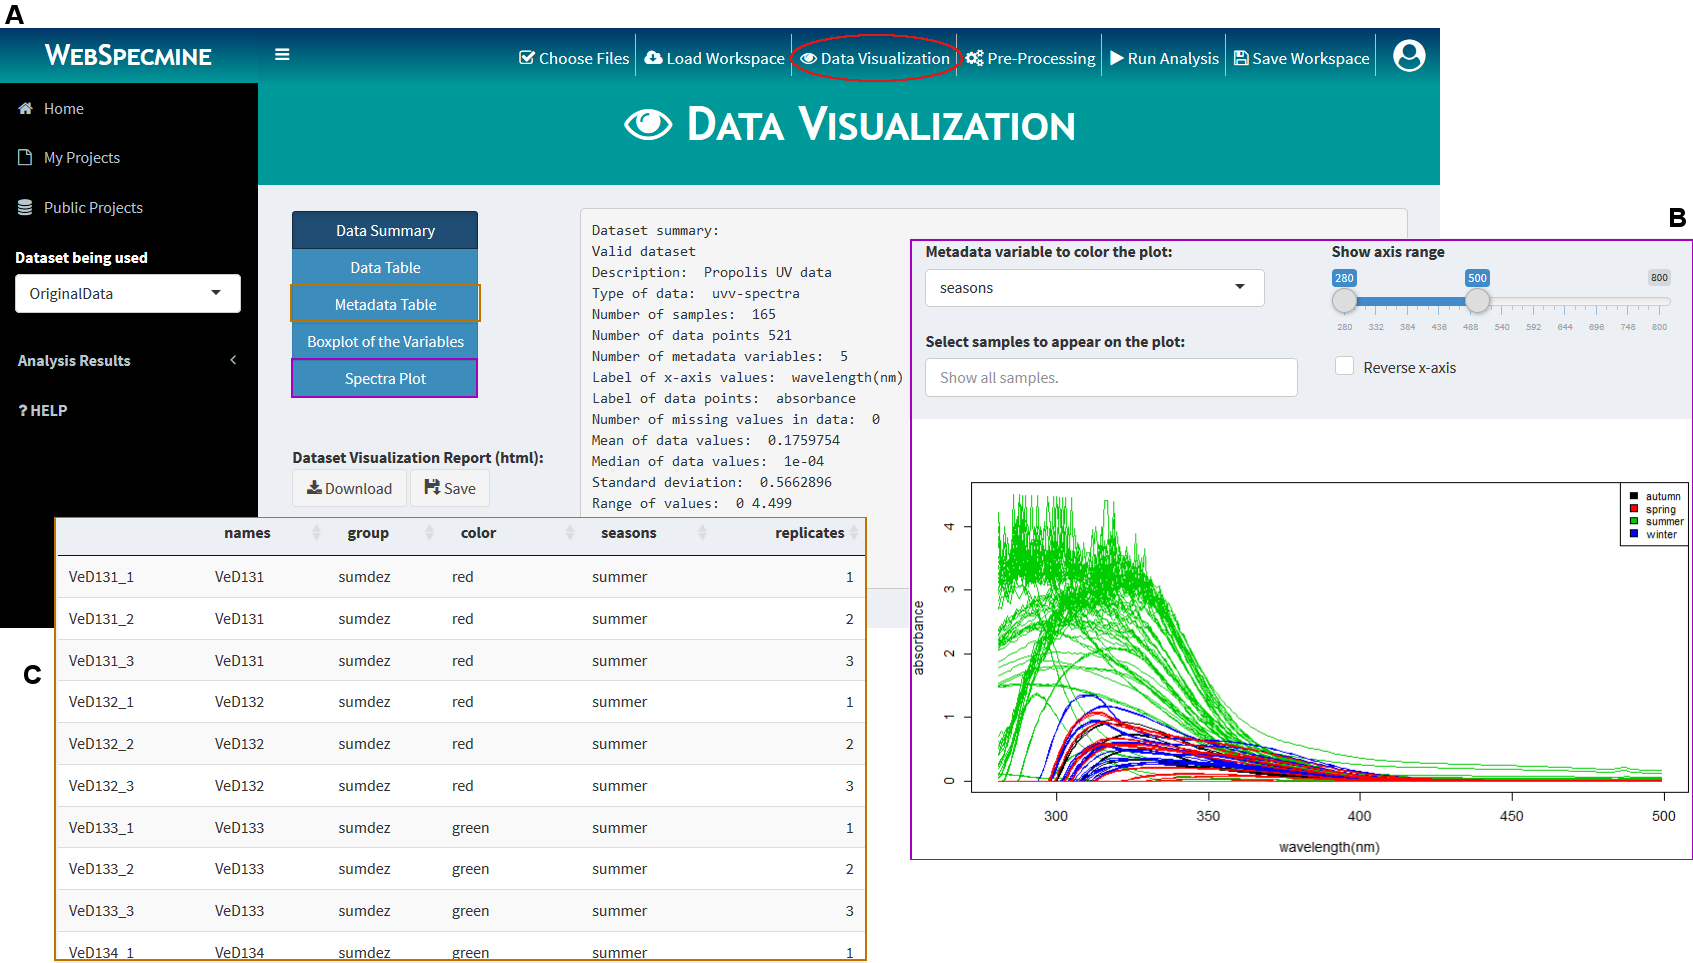
\includegraphics[width=1\linewidth]{Imagens/Propolis/data_overview}
	\caption{The \textit{Data Visualization} page showing the dataset summary (\textbf{A}), the spectra plot colored by the \textit{seasons} metadata variable (\textbf{B}), and the metadata table (\textbf{C}).}
	\label{propolis_data_overview}
\end{figure}


\subsection{Pre-processing}


To apply pre-processing methods to the dataset we go over to the \textit{Pre-Processing} page. Here, four pre-processing methods will be applied, including smoothing interpolation followed by background, offset and baseline corrections. To apply these methods, we simply have to go to the respective method box and, after selecting the parameters accordingly, click the button on the box to apply the selected method. Finally, a name must be given to the new pre-processed dataset and the process is done (\autoref{propolis_proprocessing}).

\begin{figure}[h]
	\centering
	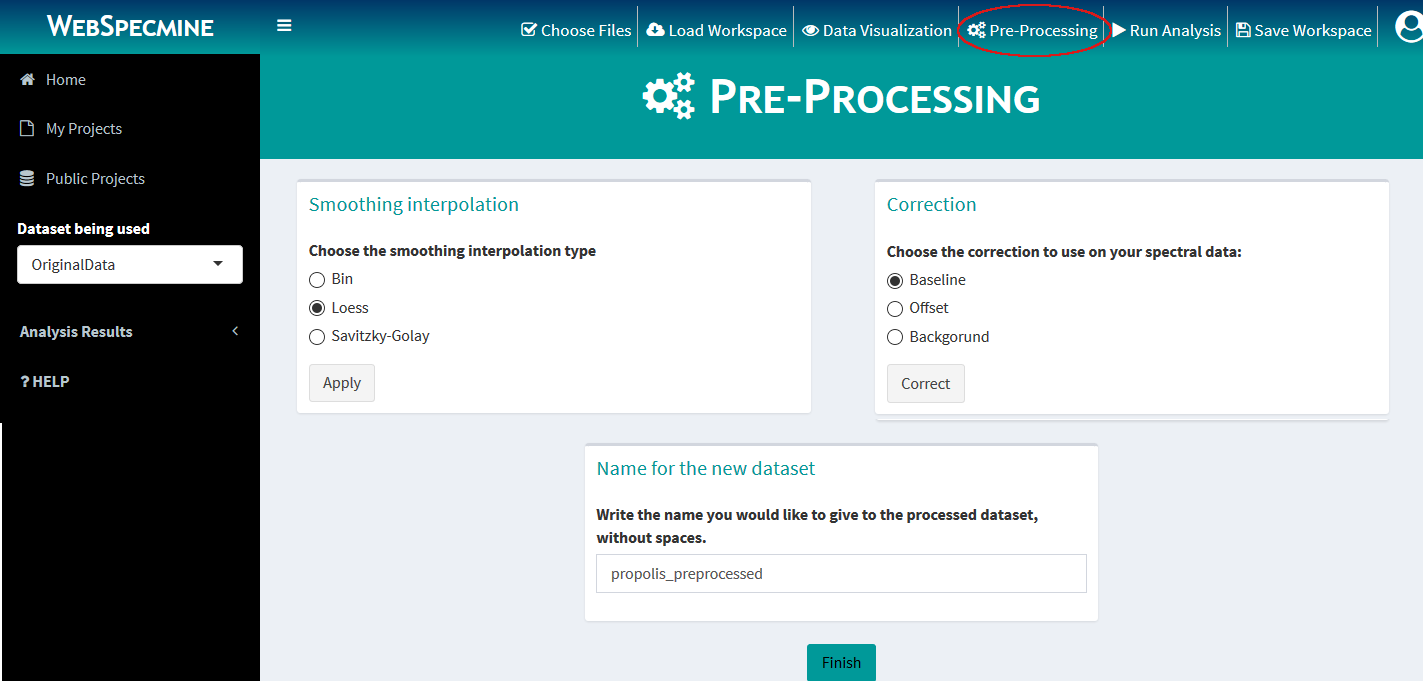
\includegraphics[width=0.8\linewidth]{Imagens/Propolis/proprocessing}
	\caption{The \textit{Pre-Processing} page emphasizing the boxes for smoothing interpolation, background, offset and baseline corrections. Please note the image was edited to emphasize the pre-processing methods used in this example.}
	\label{propolis_proprocessing}
\end{figure}


Returning back to the \textit{Data Visualization} page, the effects of the applied pre-processing methods are noticeable (\autoref{propolis_data_overview_preproc}).


\begin{figure}[H]
	\centering
	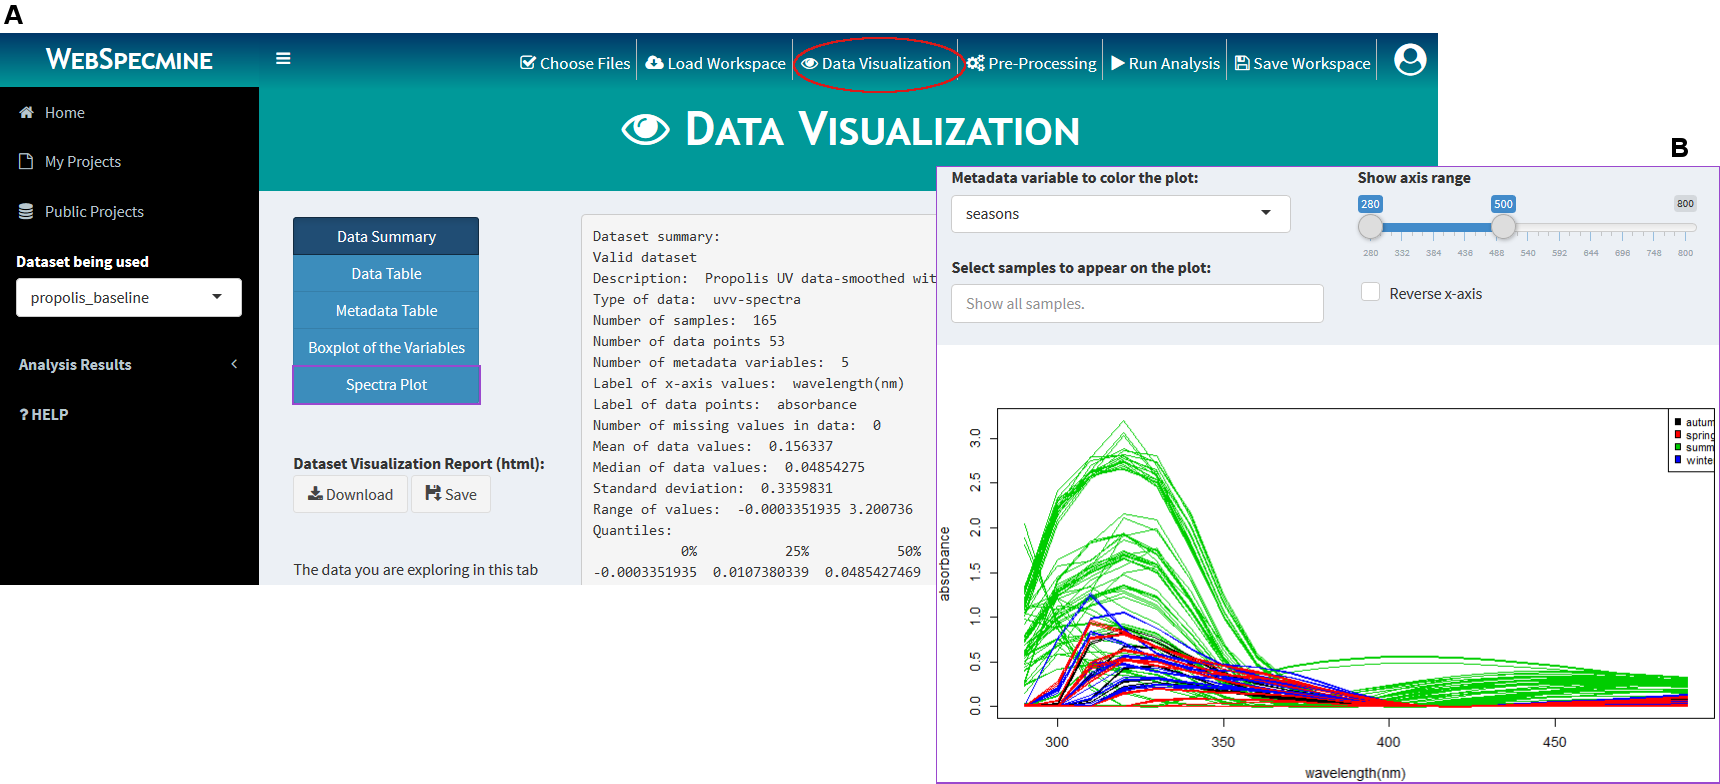
\includegraphics[width=1\linewidth]{Imagens/Propolis/data_overview_preproc}
	\caption{The \textit{Data Visualization} page showing the dataset summary (\textbf{A}) and the spectra plot colored by the \textit{seasons} metadata variable (\textbf{B}) after data pre-processing.}
	\label{propolis_data_overview_preproc}
\end{figure}



\subsection{Univariate Analysis}

The next step is to perform univariate statistical analysis, in this case one-way \gls{anova} given that the \textit{seasons} metadata variable has more than two possible values.
To perform an \gls{anova}, we must go to the \textit{Run Analysis} page and from here select the \textit{Univariate Analysis} box, leading into the analysis page (\autoref{propolis_anova}A). After selecting the analysis options and clicking \textit{Submit}, the analysis is performed and a new page appears with the analysis results (\autoref{propolis_anova}B). This analysis can be accessed anytime by clicking the respective name in the \textit{Analysis Results} menu on the sidebar. In this case, a One-way \gls{anova} with a post-hoc Tukey's \gls{hsd} was performed.

\begin{figure}[H]
	\centering
	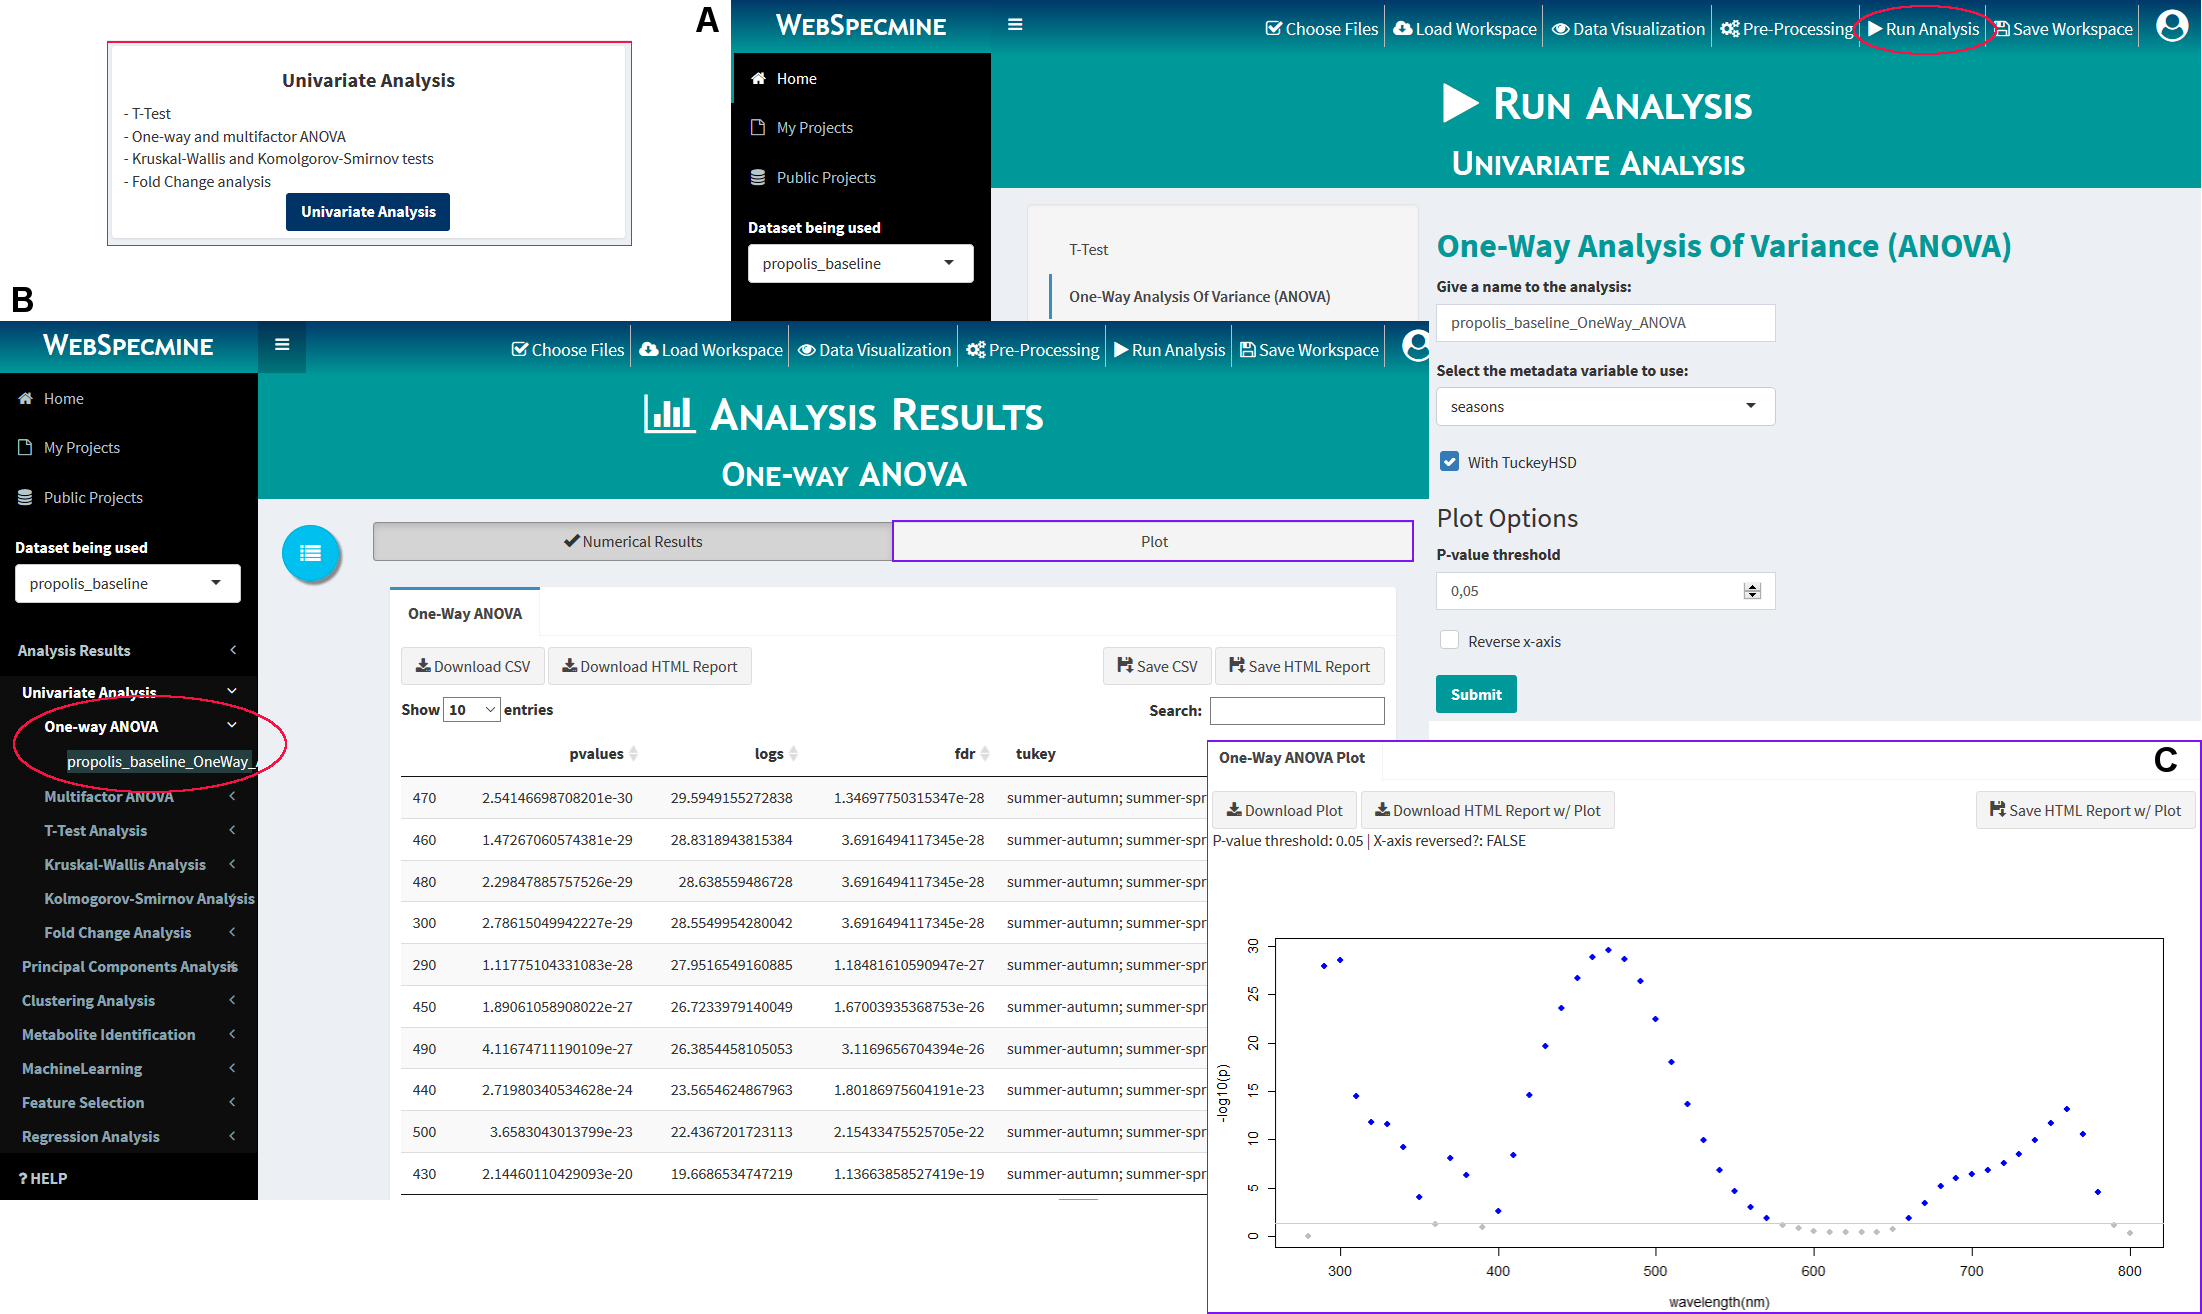
\includegraphics[width=1\linewidth]{Imagens/Propolis/anova}
	\caption{\textit{Run Analysis} page for \gls{anova} (\textbf{A}), and respective results page (\textbf{B}) showing the table results with Tukey's \gls{hsd} for the \textit{seasons} metadata variable. The \gls{anova} plot is also shown, with a defined p-value threshold of 0.05 (horizontal line) (\textbf{C}).}
	\label{propolis_anova}
\end{figure}

The results above indicate that wavelengths between 400 to 500 $\eta m$  appear to have a significant effect on the discrimination of propolis samples over the seasons.

\subsection{Clustering}

Next, we move to multivariate analysis, and an \acrlong{hca} with Euclidean distance measure and complete agglomeration method over the propolis dataset was performed. This type of analysis can be accessed through the \textit{Clustering Analysis} box in the \textit{Run Analysis} page (\autoref{propolis_hca}A). After selecting the desired values for each parameter and pressing \textit{Submit}, the analysis is performed and a new page appears with the analysis results (\autoref{propolis_hca}B). This analysis can be accessed similarly to the previous case.

\begin{figure}[H]
	\centering
	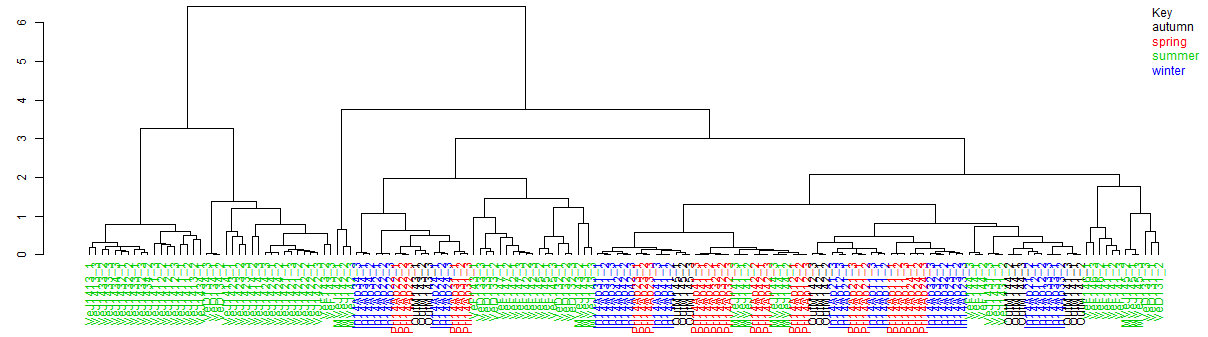
\includegraphics[width=1\linewidth]{Imagens/Propolis/hca}
	\caption{\textit{Run Analysis} page for \gls{hca} (\textbf{A}) and respective results page showing the \gls{hca} dendrogram colored according to the \textit{seasons} metadata variable (\textbf{B}). Euclidean distance and a complete agglomeration method were used.}
	\label{propolis_hca}
\end{figure}

The resulting tree (\autoref{propolis_hca}B) revealed samples discriminated into two main groups, one having samples collected in the four seasons, but with few samples collected in the summer. The other group, however, contains mostly propolis samples produced in the summer, revealing an interesting separation.


\subsection{Principal Components Analysis}

Finally, a \gls{pca} was also performed over the propolis dataset. This analysis can be accessed through the \textit{Principal Components Analysis} box in the \textit{Run Analysis} page (\autoref{propolis_pca}A). 
In this case, the we used centering by mean and scaling by standard deviation, with a pre-defined total of 10 components set. The component importance results are shown in \autoref{propolis_pca}B, also including the pairs plot for the first five components (\autoref{propolis_pca}D) and a 3D scores plot (\autoref{propolis_pca}E), both colored according to the \textit{seasons} metadata variable. \autoref{propolis_pca}C shows the \textit{Make plots} tab for the scree plot. These results may be accessed at any time, similarly to the previous cases.

\begin{figure}[H]
	\centering
	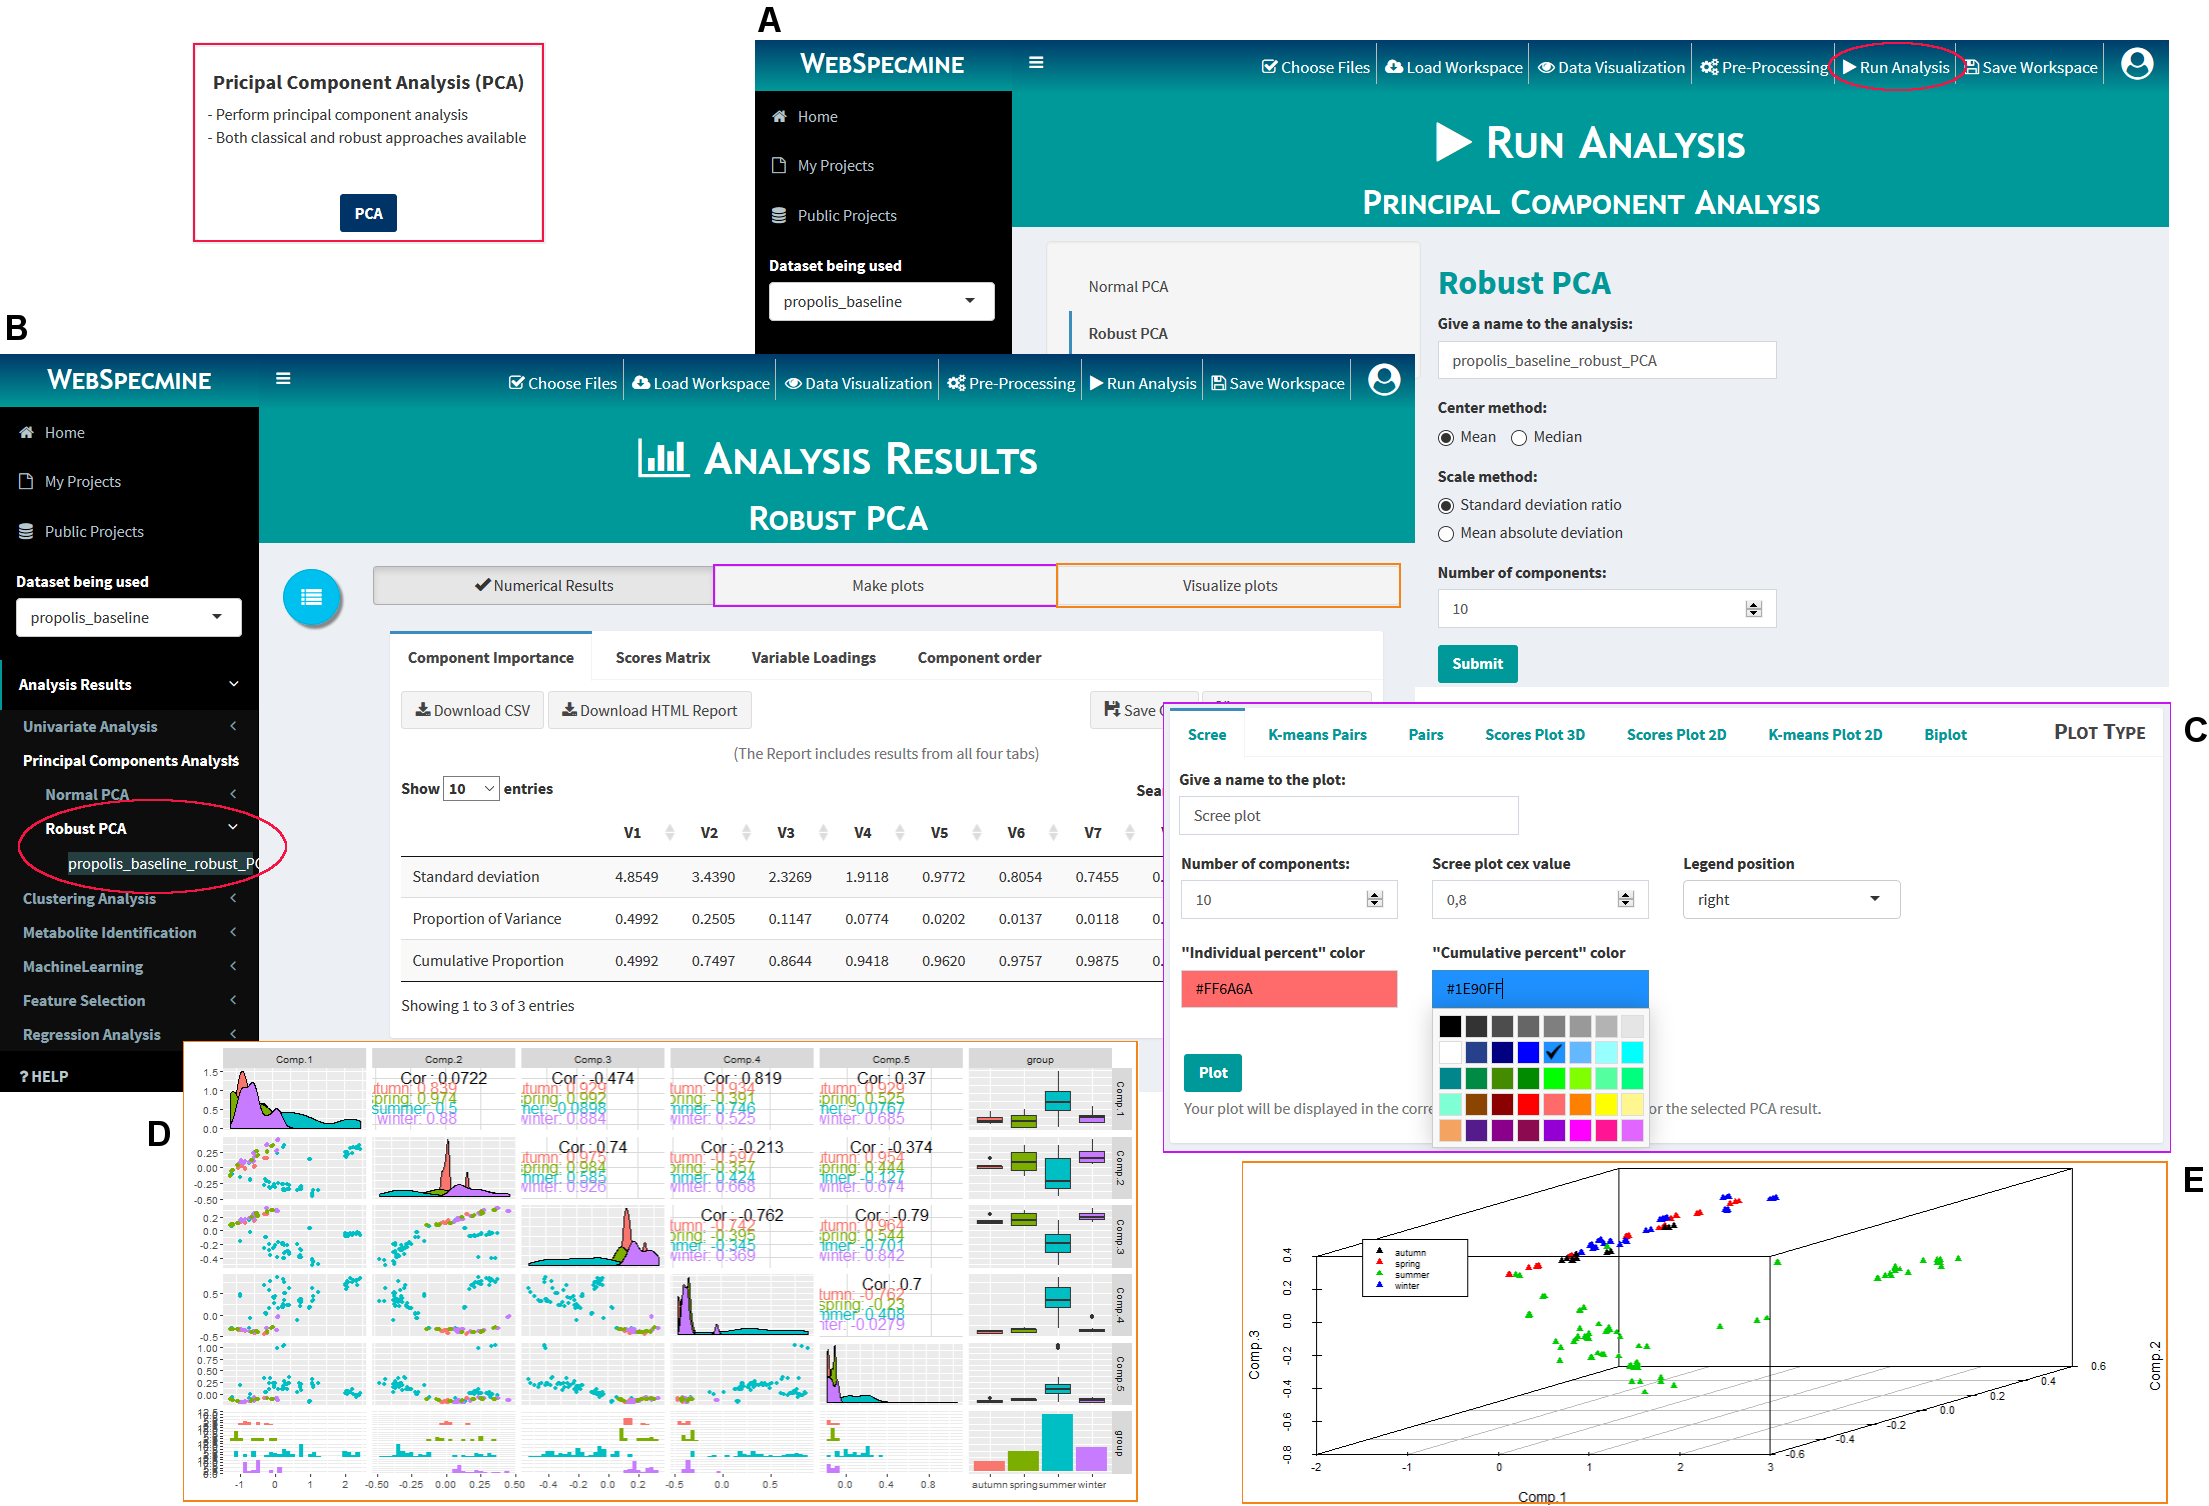
\includegraphics[width=1\linewidth]{Imagens/Propolis/pca}
	\caption{\textit{Run Analysis} page for \gls{pca} (\textbf{A}) and respective results page showing the component importance table (\textbf{B}), the \textit{Make plots} tab for the scree plot (\textbf{C}), and a pairs plot for the first five components (\textbf{D}) and a 3D scores plot (\textbf{E}), both colored according to the \textit{seasons} metadata variable.}
	\label{propolis_pca}
\end{figure}


The first two components PC1 (50\%) and PC2 (25.05\%) explained about 75.05\% of the total variance of the dataset (\autoref{propolis_pca}B). In general, the results of \gls{pca} and \gls{hca} are complementary, by confirming the sample discrimination by seasons into two groups (\autoref{propolis_pca}D, \autoref{propolis_pca}E). 

The raw data and full analysis report performed using the \textit{specmine} package for this study can be accessed at \href{http://darwin.di.uminho.pt/metabolomicspackage/propolis-sj.html}{\nolinkurl{http://darwin.di.uminho.pt/metabolomicspackage/propolis-sj.html}}.




\section{Cassava's post-harvest physiological deterioration}

\subsection{Context}

The \textit{cassava} crop (\textit{Manihot esculenta}) is characterized by its starchy roots, being considered a staple food and animal feed in tropical and sub-tropical areas. As a tropical root crop, it undergoes \acrfull{ppd}, both physiological (or primary deterioration) and microbiological (or secondary deterioration). This process is characterized by the appearance of blue–black streaks in the root vascular tissue, which later spread, causing a more general brown discoloration, unsatisfactory cooking qualities, and adverse taste. \gls{ppd} begins quickly within 24h post-harvest, limiting the marketability of the roots, and they need, therefore, to be consumed shortly after harvesting.

The aim of the present study was to identify and discriminate changes in the chemical and enzymatic composition of cassava genotypes samples during post-harvest deterioration, with the aid of supervised and unsupervised methods of data analysis.

For this, samples with different stages of deterioration were collected, more specifically fresh samples (0 days) and samples with 3 days, 5 days, 8 days and 11 days of deterioration (\gls{ppd}). Additionally, the samples collected were from four different varieties: SCS 253 Sangão (SAN); Branco (BRA); IAC576-70 - \textit{Instituto Agronômico de Campinas} (IAC); and Oriental (ORI). A total of 80 samples were collected (16 samples with 5 replicates each) and the \gls{ir} transmittance spectra recorded over a spectral window from 4000 to 400 $cm^{-1}$ \citep{uarrota2014metabolomics}.


\subsection{Data Loading}

In this case, the dataset will be directly created from the user's local computer files, without the need of authentication, unlike in \autoref{propolis_loading} where it was assumed the user would be logged in and already had the files uploaded in a project on the web platform. The main difference compared to when the user is logged is the fact that there aren't any saved projects ready to import as a dataset, hence the need to import the files containing the data directly from the computer. Additionally, the workspace cannot be saved to later resume the analysis and while reports can still be generated and downloaded, they cannot be saved into the users personal project library. 

To create the dataset, we start by clicking the \textit{New Project} button on the header. A new window appears with fields to upload both data and metadata files and to specify each file's options accordingly (\autoref{cassava_create_project}A). The DX files from this study are stored in a ZIP folder, which can be uploaded directly using the specified field (\autoref{cassava_create_project}B).

\begin{figure}[h]
	\centering
	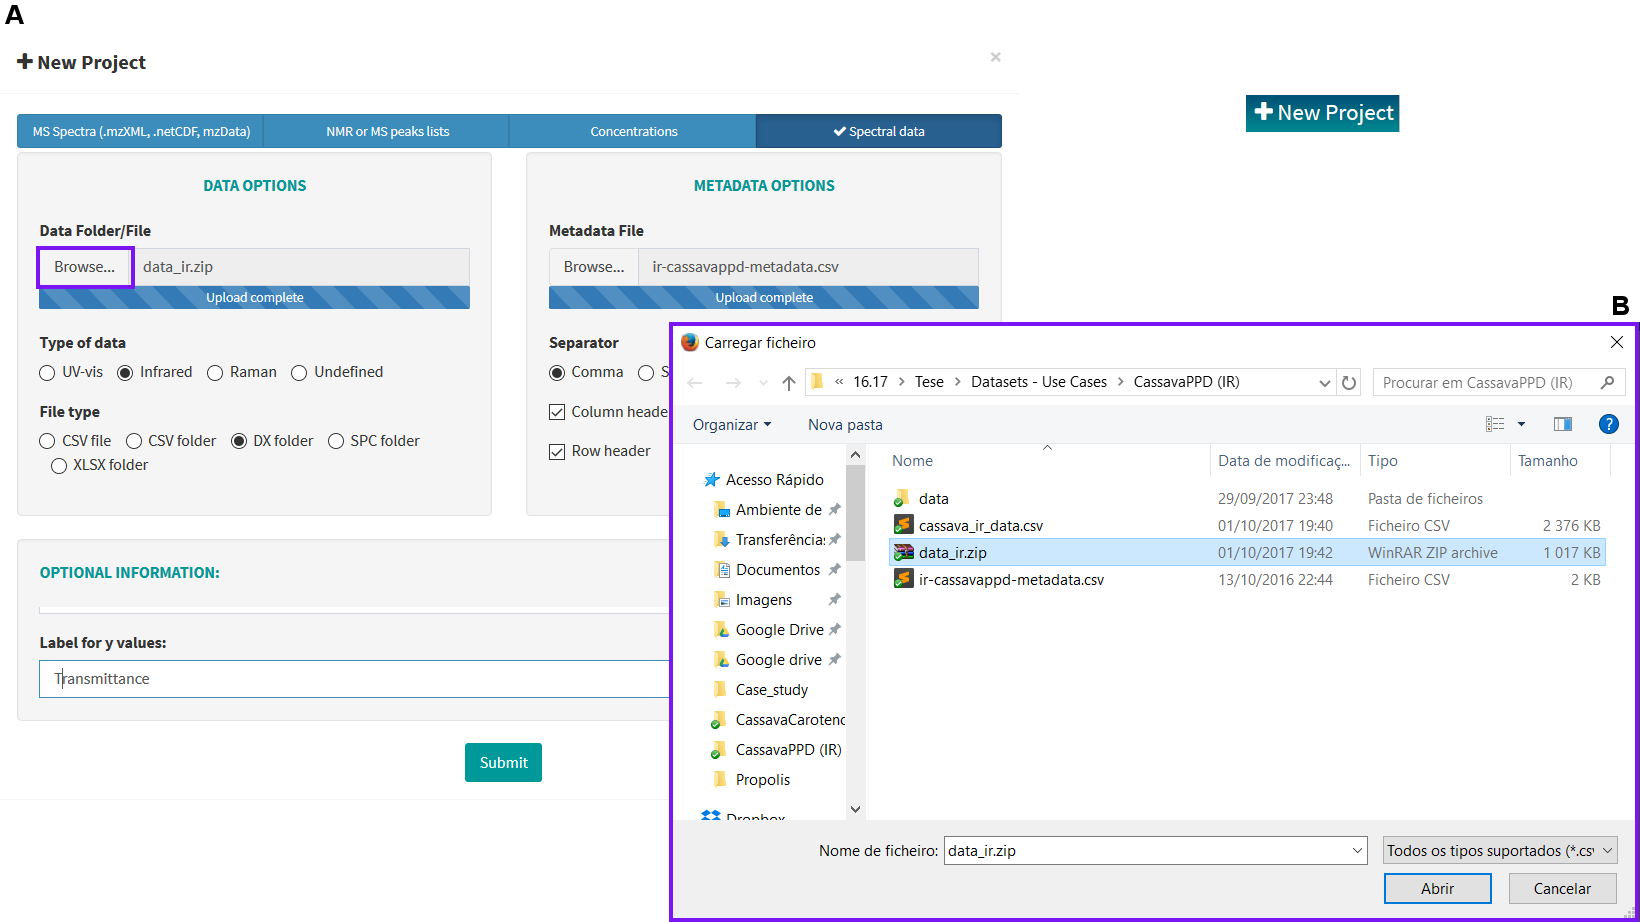
\includegraphics[width=1\linewidth]{Imagens/CassavaPPD/data_load}
	\caption{Upon clicking the \textit{New Project} button on the header a window appears with fields to upload both data and metadata files and to specify each files options accordingly (\textbf{A}). In this case, a zip folder containing DX files is being uploaded (\textbf{B}).}
	\label{cassava_create_project}
\end{figure}


\subsection{Data Overview}

Once the dataset is created, its information can be easily accessed in the \textit{Data Visualization} page. In \autoref{cassava_data_overview}, the summary of the propolis dataset, along with the spectra plot colored by the \textit{varieties} metadata variable and the first 11 rows of the metadata table are shown. The \gls{ir} dataset has 3 metadata variables, a total of 80 samples and about 3735 data points, with no missing values.

\begin{figure}[h]
	\centering
	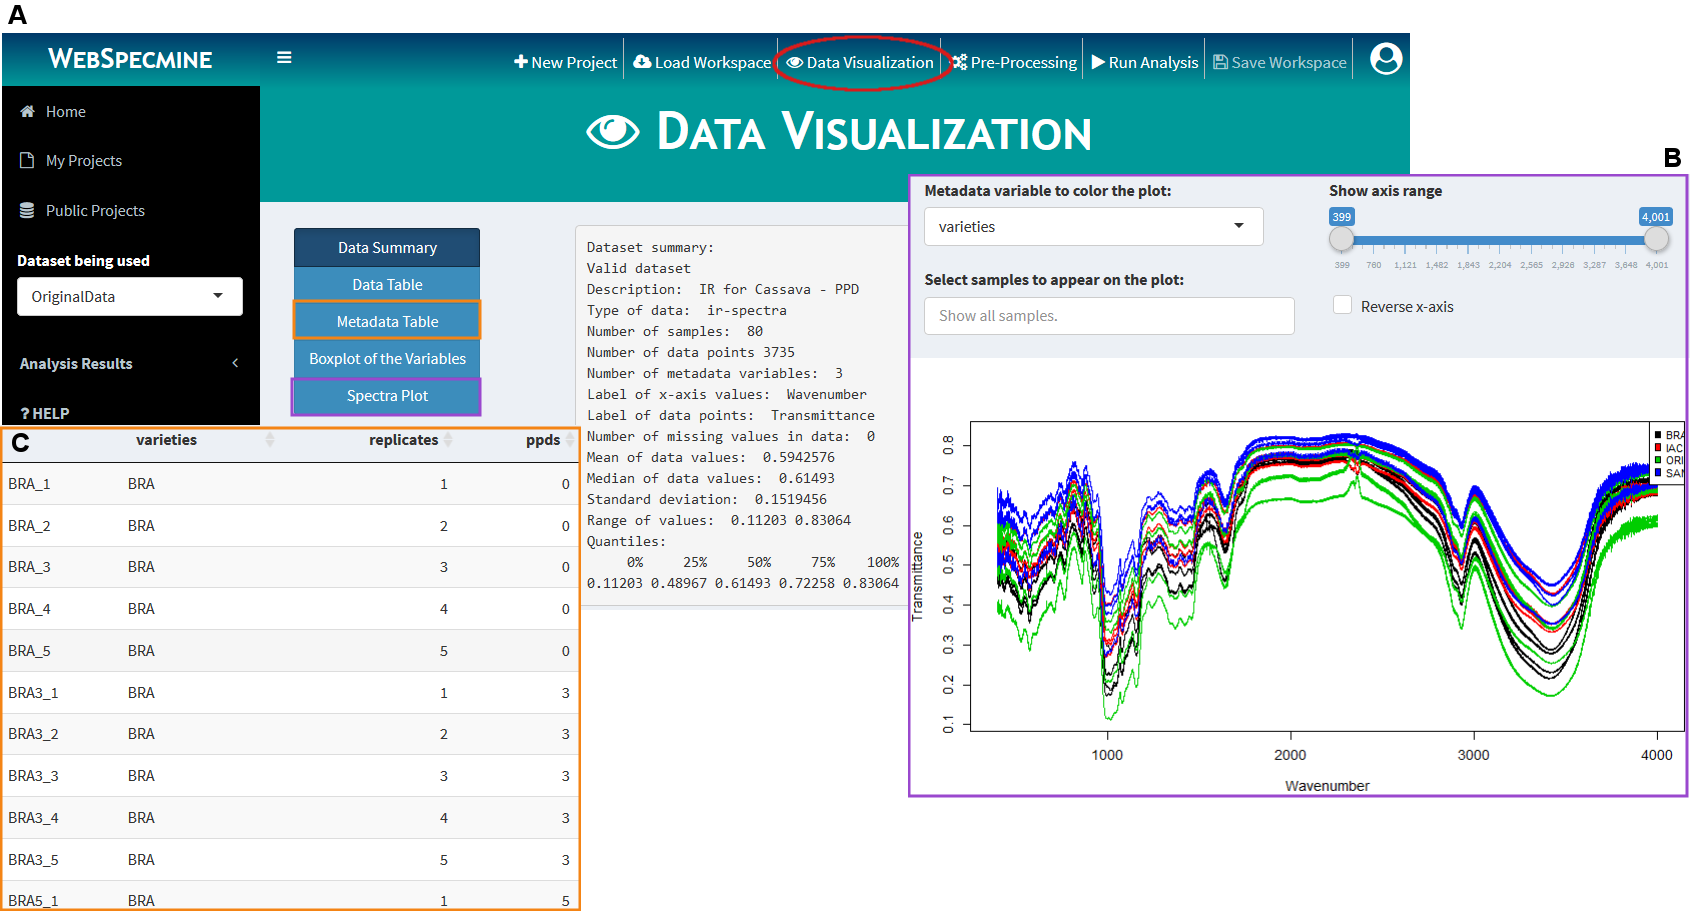
\includegraphics[width=1\linewidth]{Imagens/CassavaPPD/data_overview}
	\caption{The \textit{Data Visualization} page showing the dataset summary (\textbf{A}), the spectra plot colored by the \textit{varieties} metadata variable (\textbf{B}) and the first 11 rows of metadata table (\textbf{C}).}
	\label{cassava_data_overview}
\end{figure}


\subsection{Pre-processing}

The pre-processing methods used in this study consisted in converting the \textit{ppd} metadata variable to factor, the aggregation of replicates and applying smoothing interpolation. All these methods can be easily applied over the dataset on the \textit{Pre-Processing} page by going the respective method box and, after selecting the parameters accordingly, click the button on the box to apply the selected method. 
As before, a name must be given to the new dataset and the process is done (\autoref{cassava_preprocessing}).

\begin{figure}[H]
	\centering
	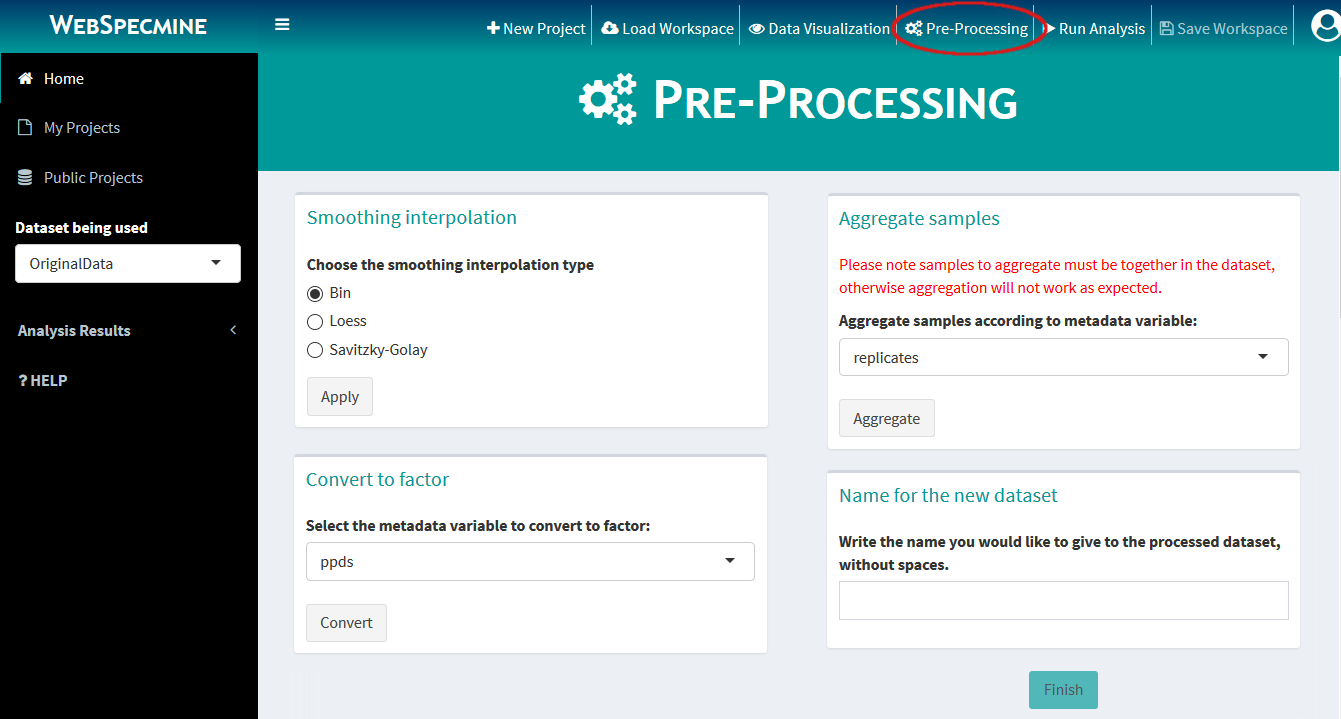
\includegraphics[width=0.8\linewidth]{Imagens/CassavaPPD/preprocessing}
	\caption{The \textit{Pre-Processing} page emphasizing the boxes for smoothing interpolation, conversion to factor and sample aggregation. Please note the image was edited to emphasize the pre-processing methods used in this example.}
	\label{cassava_preprocessing}
\end{figure}


From the \textit{Data Visualization} page the effects of the applied pre-processing methods are noticeable (\autoref{cassava_summary_preprocessing}A). The dataset now has 16 samples, 1868 data points and 2 metadata variables. The \textit{ppd} metadata variable, as a factor, can now be used to color the plot (\autoref{cassava_summary_preprocessing}B).

\begin{figure}[H]
	\centering
	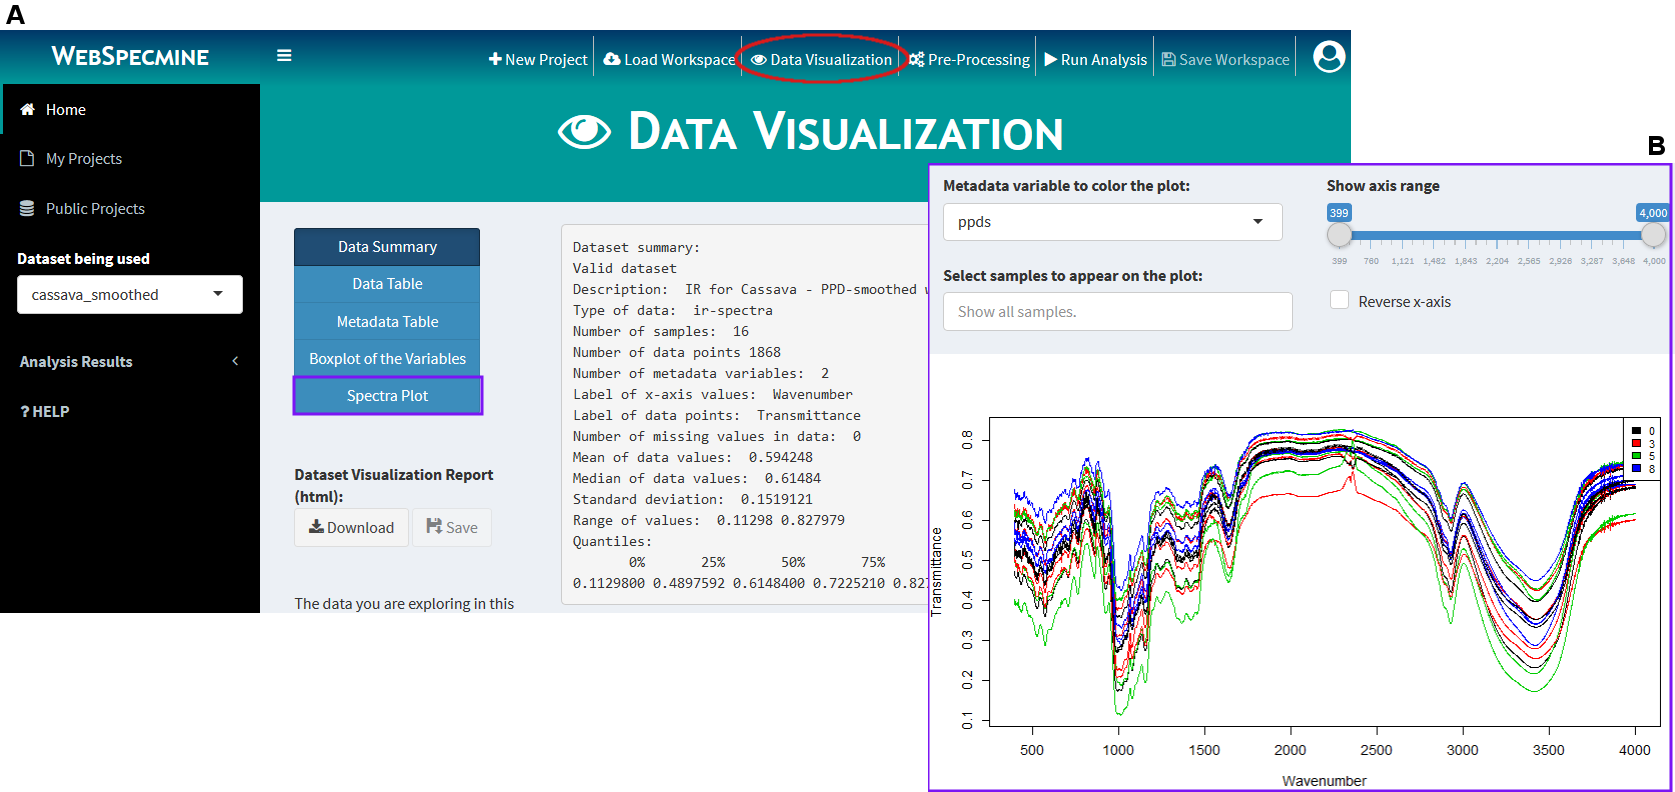
\includegraphics[width=1\linewidth]{Imagens/CassavaPPD/data_overview_preproc}
	\caption{The \textit{Data Visualization} page showing the dataset summary (\textbf{A}) and the spectra plot colored by the \textit{ppd} metadata variable (\textbf{B}) after data pre-processing.}
	\label{cassava_summary_preprocessing}
\end{figure}


\subsection{Principal Components Analysis}

A \gls{pca} was performed over the cassava dataset. This analysis can be accessed through the \textit{Principal Components Analysis} box in the \textit{Run Analysis} page (\autoref{propolis_pca}A). The data was both scaled and centered for this analysis. The component importance results are shown in \autoref{cassava_pca}B, also including the pairs plot for the first five components (\autoref{propolis_pca}C), the K-means pairs plot for the first 5 components (3 clusters) (\autoref{propolis_pca}D) and the distribution of the 16 samples on the first and second \gls{pca} components on a scored plot using the \textit{ppd} metadata variable (\autoref{propolis_pca}E). 


\begin{figure}[H]
	\centering
	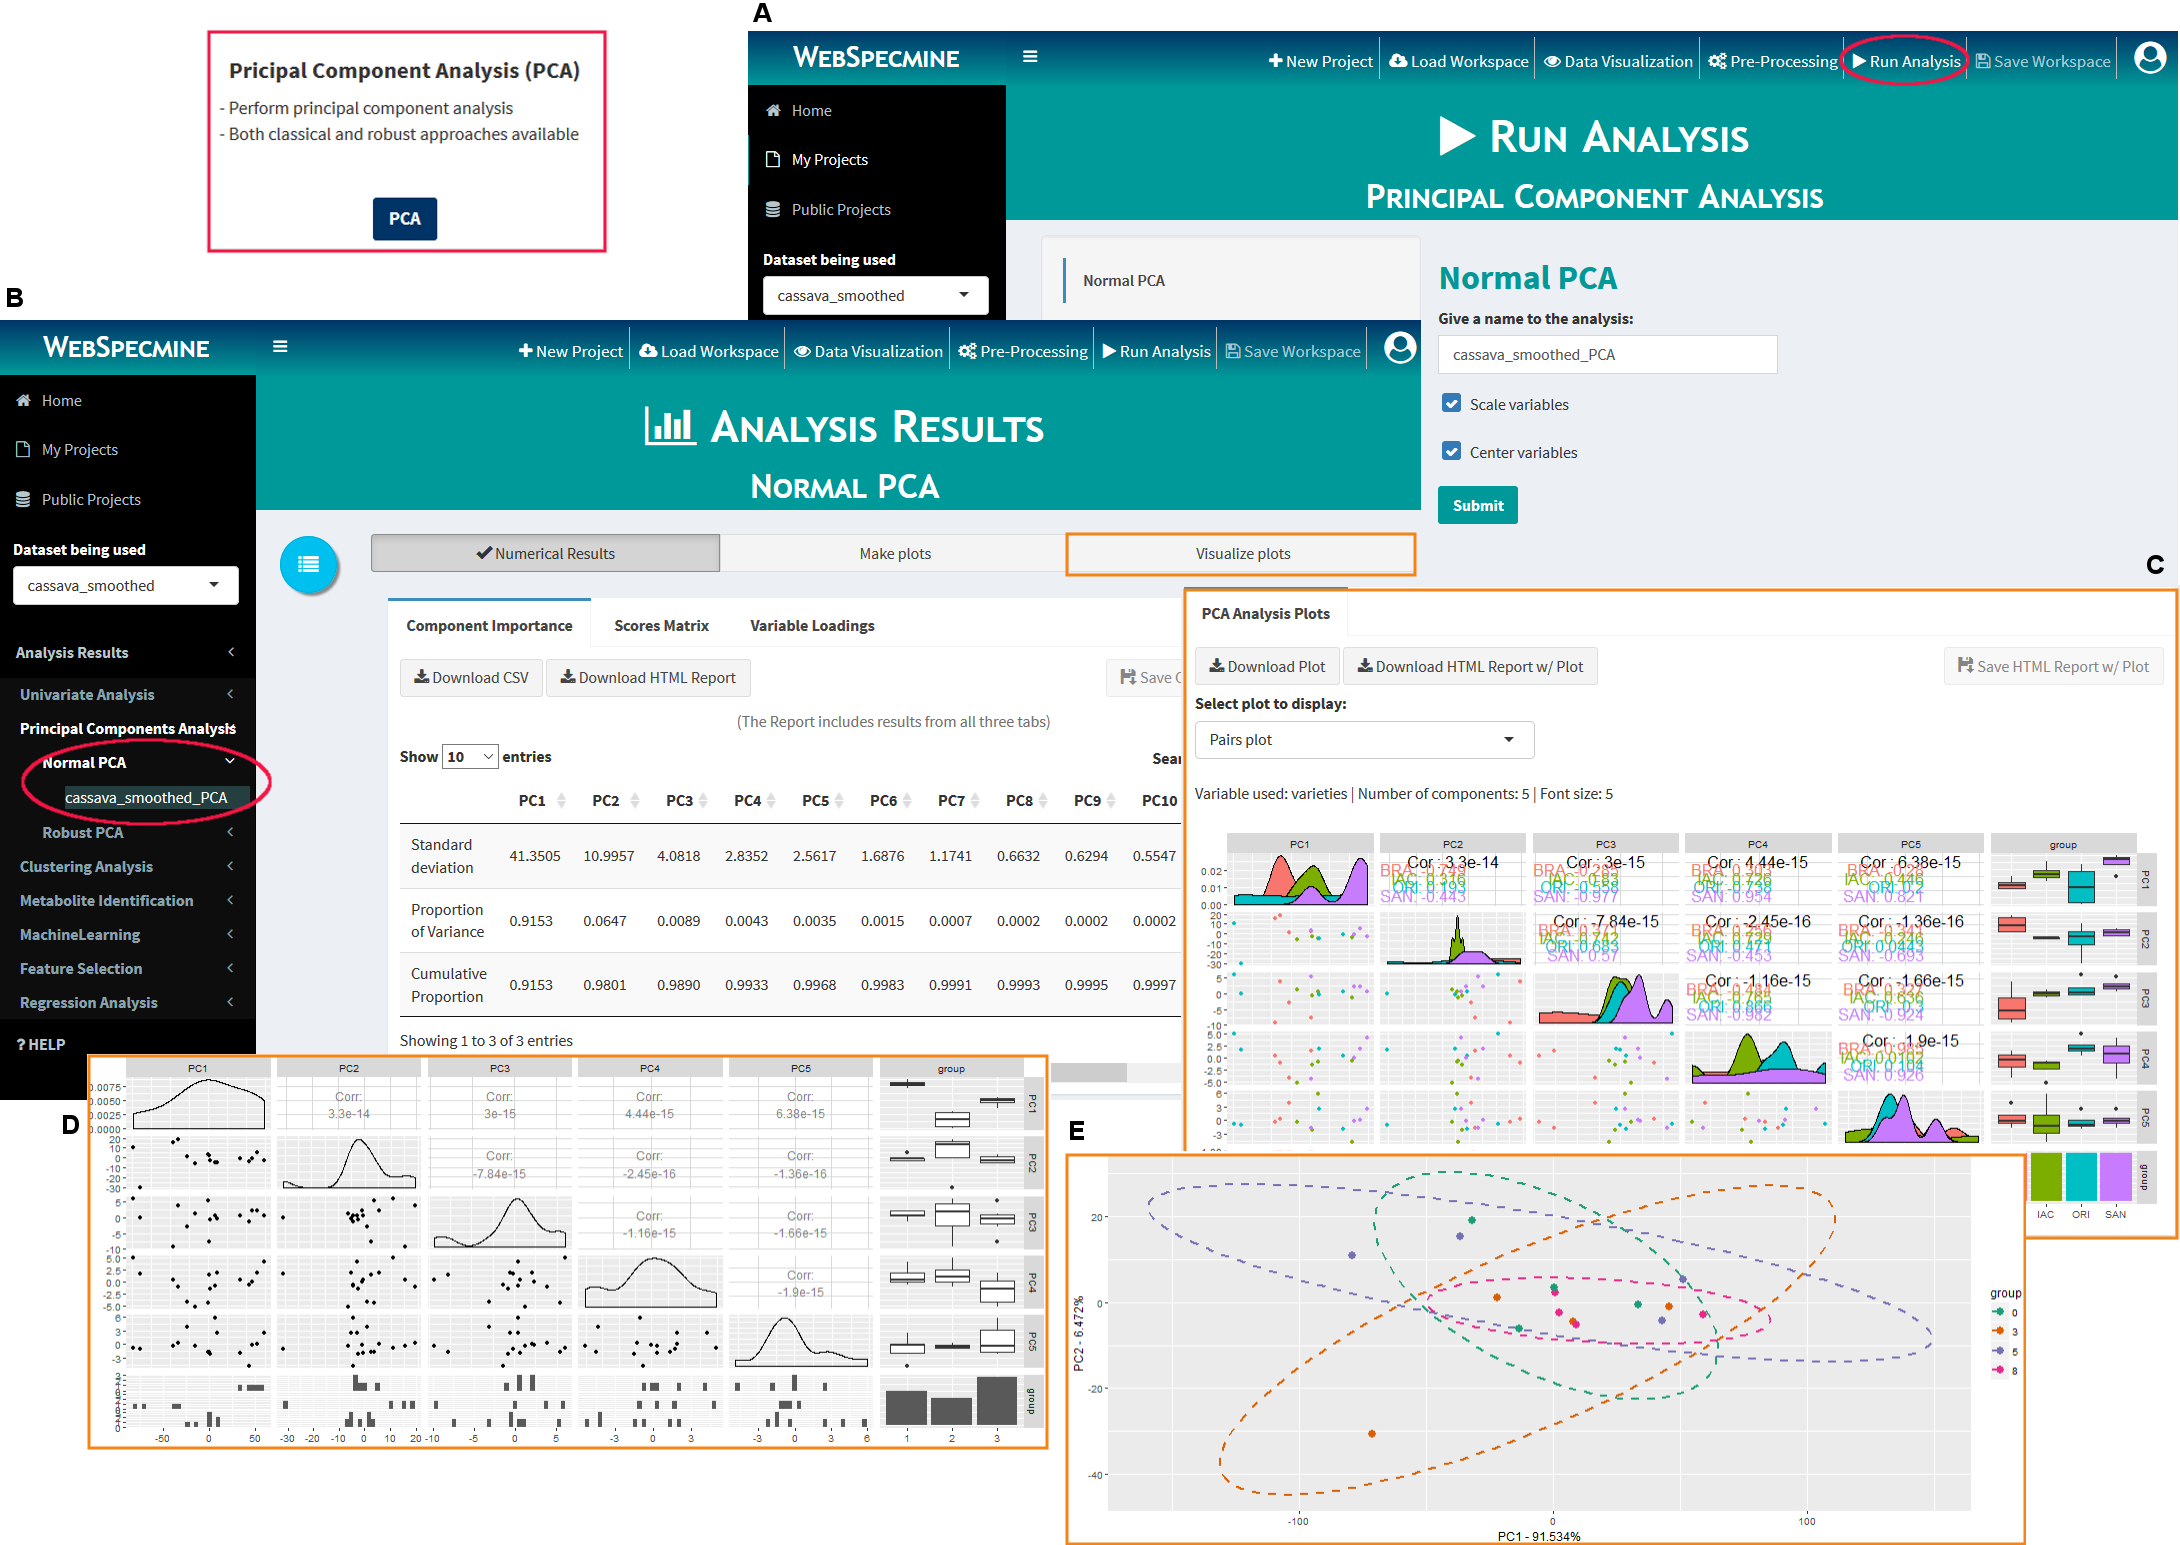
\includegraphics[width=1\linewidth]{Imagens/CassavaPPD/pca}
	\caption{\textit{Run Analysis} page for \gls{pca} (\textbf{A}) and respective results page showing the component importance table (\textbf{B}), a pairs plot for the first five components (\textbf{C}), a k-means plot for the first five components (3 clusters) (\textbf{D}) and a 2D scores plot for the \textit{ppd} metadata variable (\textbf{E}).}
	\label{cassava_pca}
\end{figure}

The total variance of the data explained by the \gls{pca} model built was 98.01\%, with 91.63\% from PC1 and 6.47\% from PC2 (\autoref{cassava_pca}B). A visible separation between ORI and BRA (susceptible and tolerant \gls{ppd} genotypes, respectively) is shown, although some overlap of the samples of most genotypes was observed (\autoref{cassava_pca}C). The scores plot showed sample overlapping using the \textit{ppd} metadata variable (\autoref{cassava_pca}E).



\subsection{Correlation Analysis}

A correlation analysis was also performed over the cassava dataset. This type of analysis can be accessed through the \textit{Regression Analysis} box in the \textit{Run Analysis} page. For this analysis the Pearson correlation method was chosen, calculating the correlation between samples (\autoref{cassava_correlation}A). \autoref{cassava_correlation}B shows the resulting correlation matrix, with the corresponding generated heatmap represented in \autoref{cassava_correlation}C.


\begin{figure}[H]
	\centering
	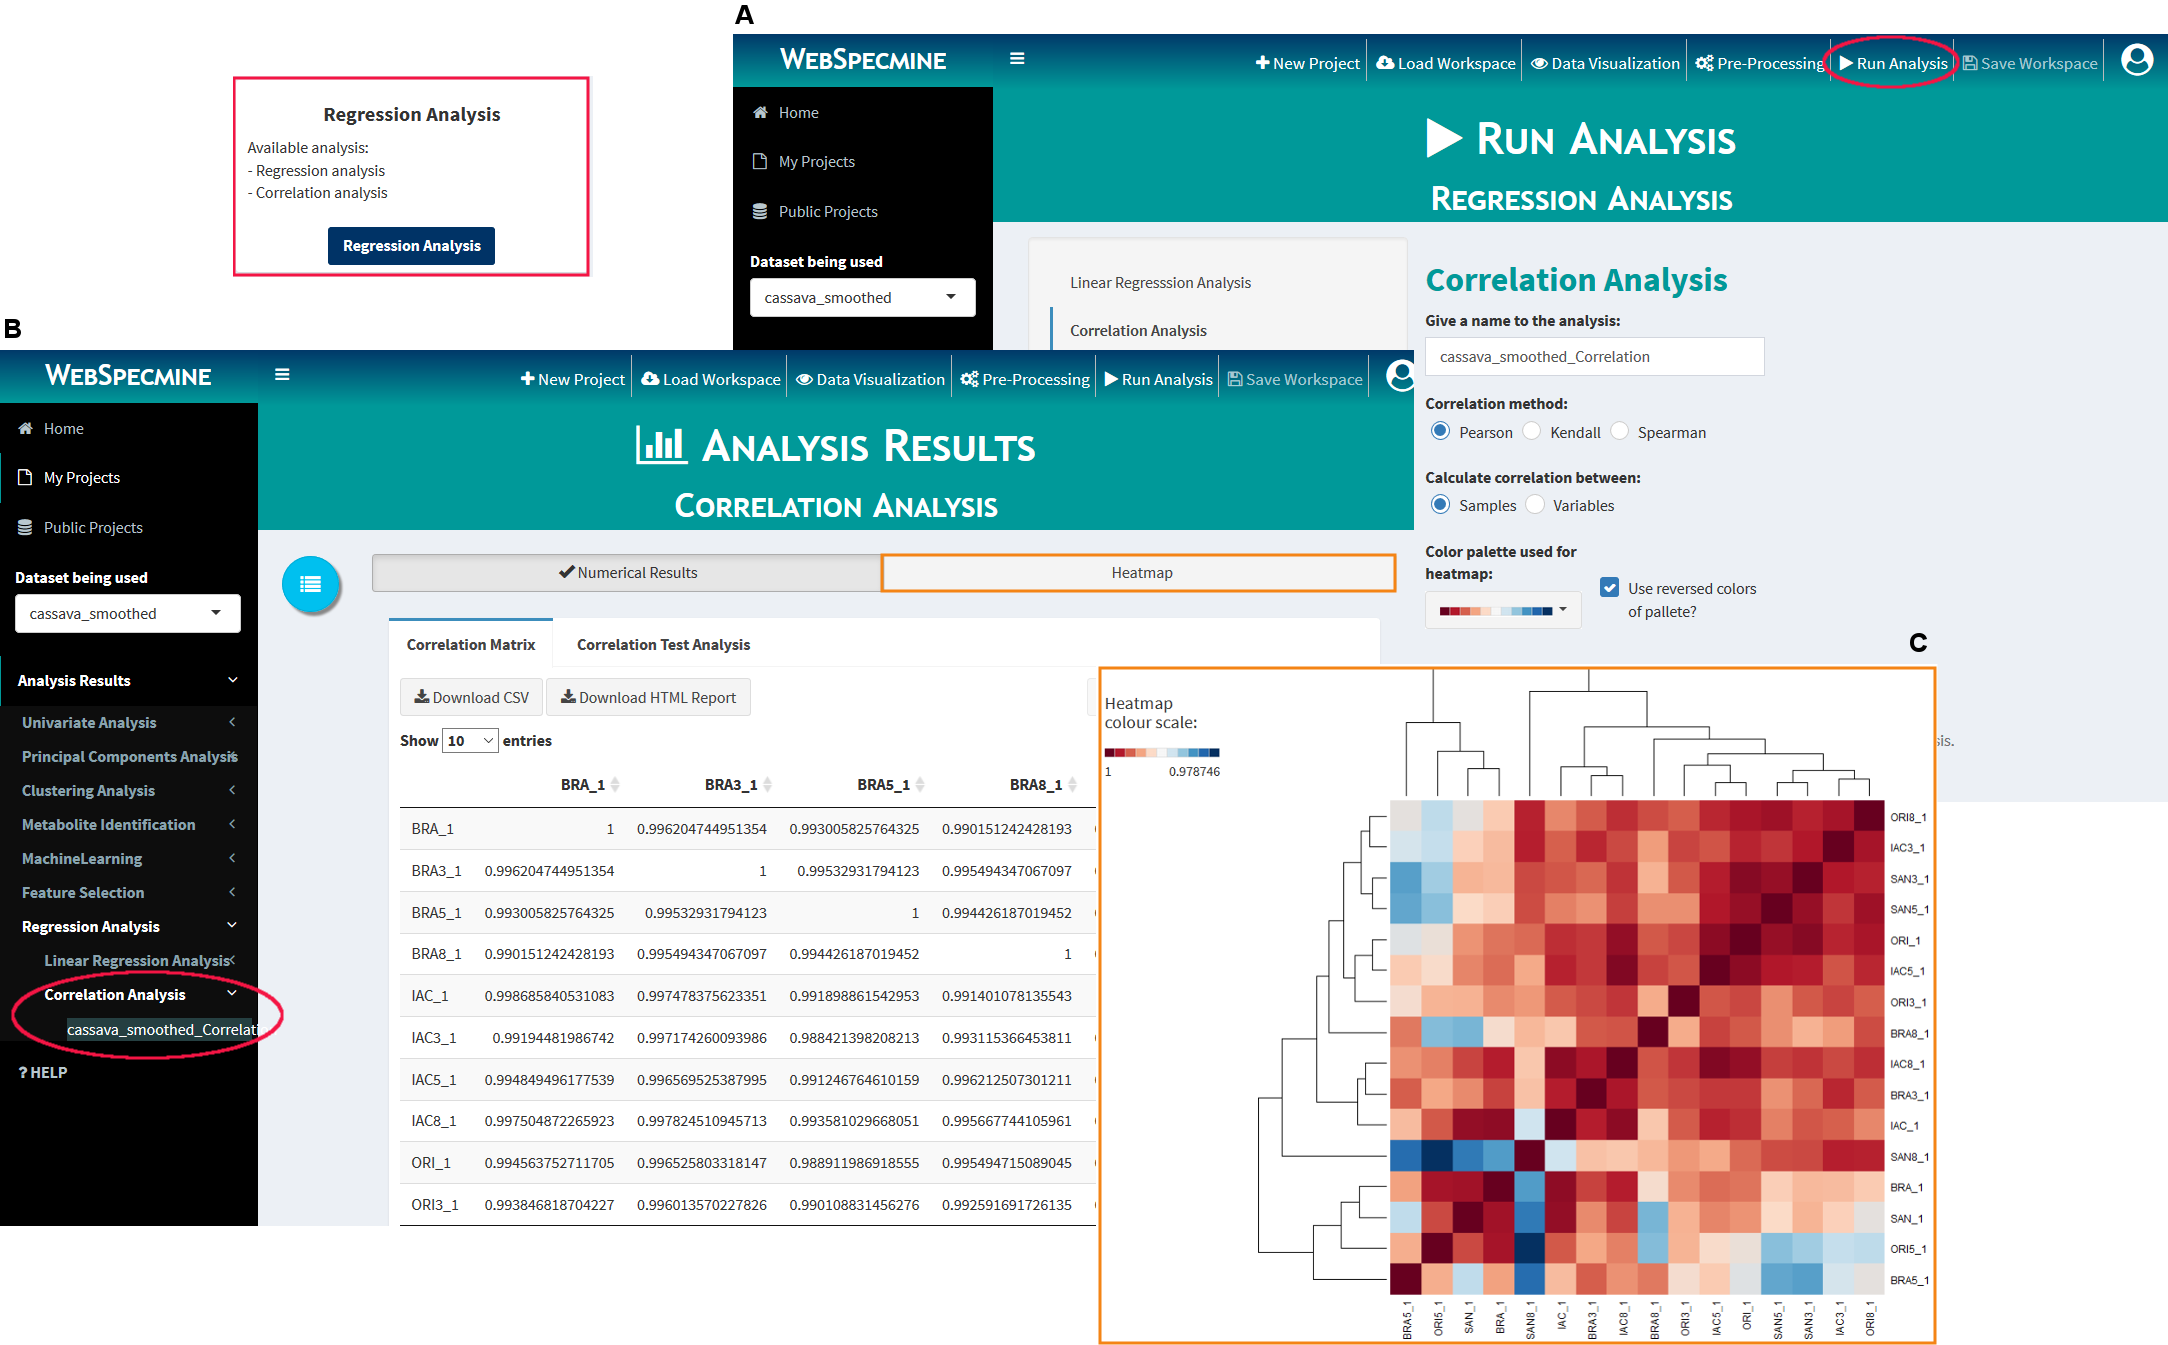
\includegraphics[width=1\linewidth]{Imagens/CassavaPPD/correlation}
	\caption{\textit{Run Analysis} page for correlation analysis (\textbf{A}) and respective results page showing the correlation matrix (\textbf{B}) and resulting heatmap correlating samples (\textbf{C}).}
	\label{cassava_correlation}
\end{figure}

The heatmap generated suggests most samples are positively correlated (\autoref{cassava_correlation}C).


\subsection{Feature Selection}

Next, a feature selection approach was performed over the dataset. To access this type of analysis, simply select the \textit{Feature Selection} box in the \textit{Run Analysis} page. Here, the \gls{rfe} method was selected, choosing random forests model to fit the data and the \textit{varieties} metadata as response variable. A 10-fold cross-validation was selected (\autoref{cassava_feature_selection}A), with 5 repetitions. In \autoref{cassava_feature_selection}B, the feature selection results are displayed, as well as the plot with the performance profile in \autoref{cassava_feature_selection}C. 


\begin{figure}[H]
	\centering
	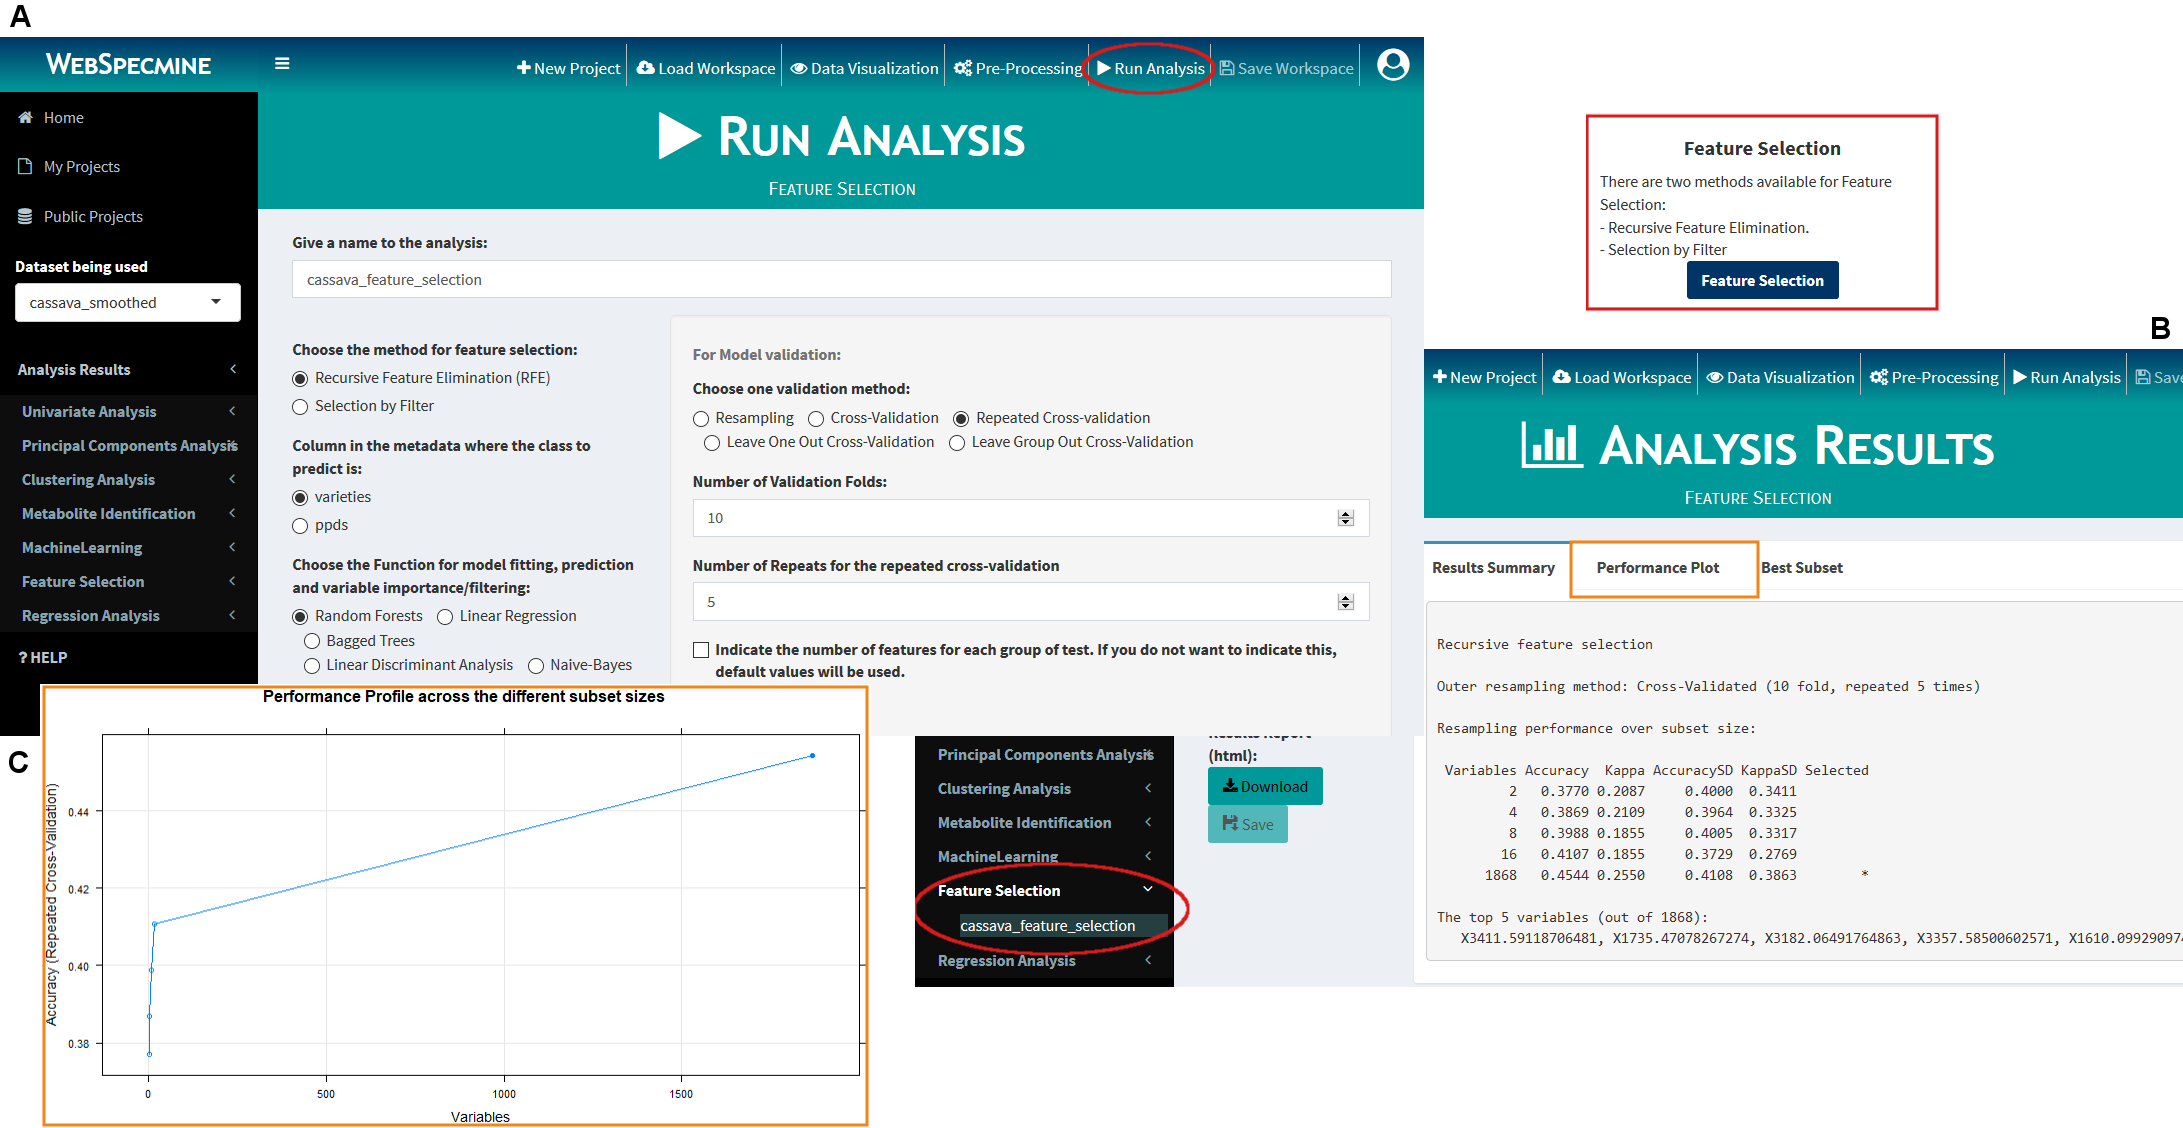
\includegraphics[width=1\linewidth]{Imagens/CassavaPPD/feature_selection}
	\caption{\textit{Run Analysis} page for feature selection analysis (\textbf{A}), and respective results page showing the performance metrics (\textbf{B}) and plot with the performance profile (\textbf{C}).}
	\label{cassava_feature_selection}
\end{figure}

The results above indicate that there is no improvement in cross-validation performance by performing feature selection, with the best accuracy being achieved when using the entire set of features.


\subsection{Machine Learning}

Finally, a machine learning analysis was performed. This type of analysis can be accessed through the \textit{Machine Learning} box in the \textit{Run Analysis} page. In this analysis, the \gls{pls} model was chosen to fit the data, using the \textit{ppd} metadata variable for class prediction. A 10-fold cross-validation was selected, with accuracy as selected performance metric (\autoref{cassava_machine_learning}A). \autoref{cassava_machine_learning}B displays the analysis' performance metrics for the \gls{pls} model, while \autoref{cassava_machine_learning}C shows the full results from the tuning parameters for this model, with the variable importance table shown in \autoref{cassava_machine_learning}D.


\begin{figure}[H]
	\centering
	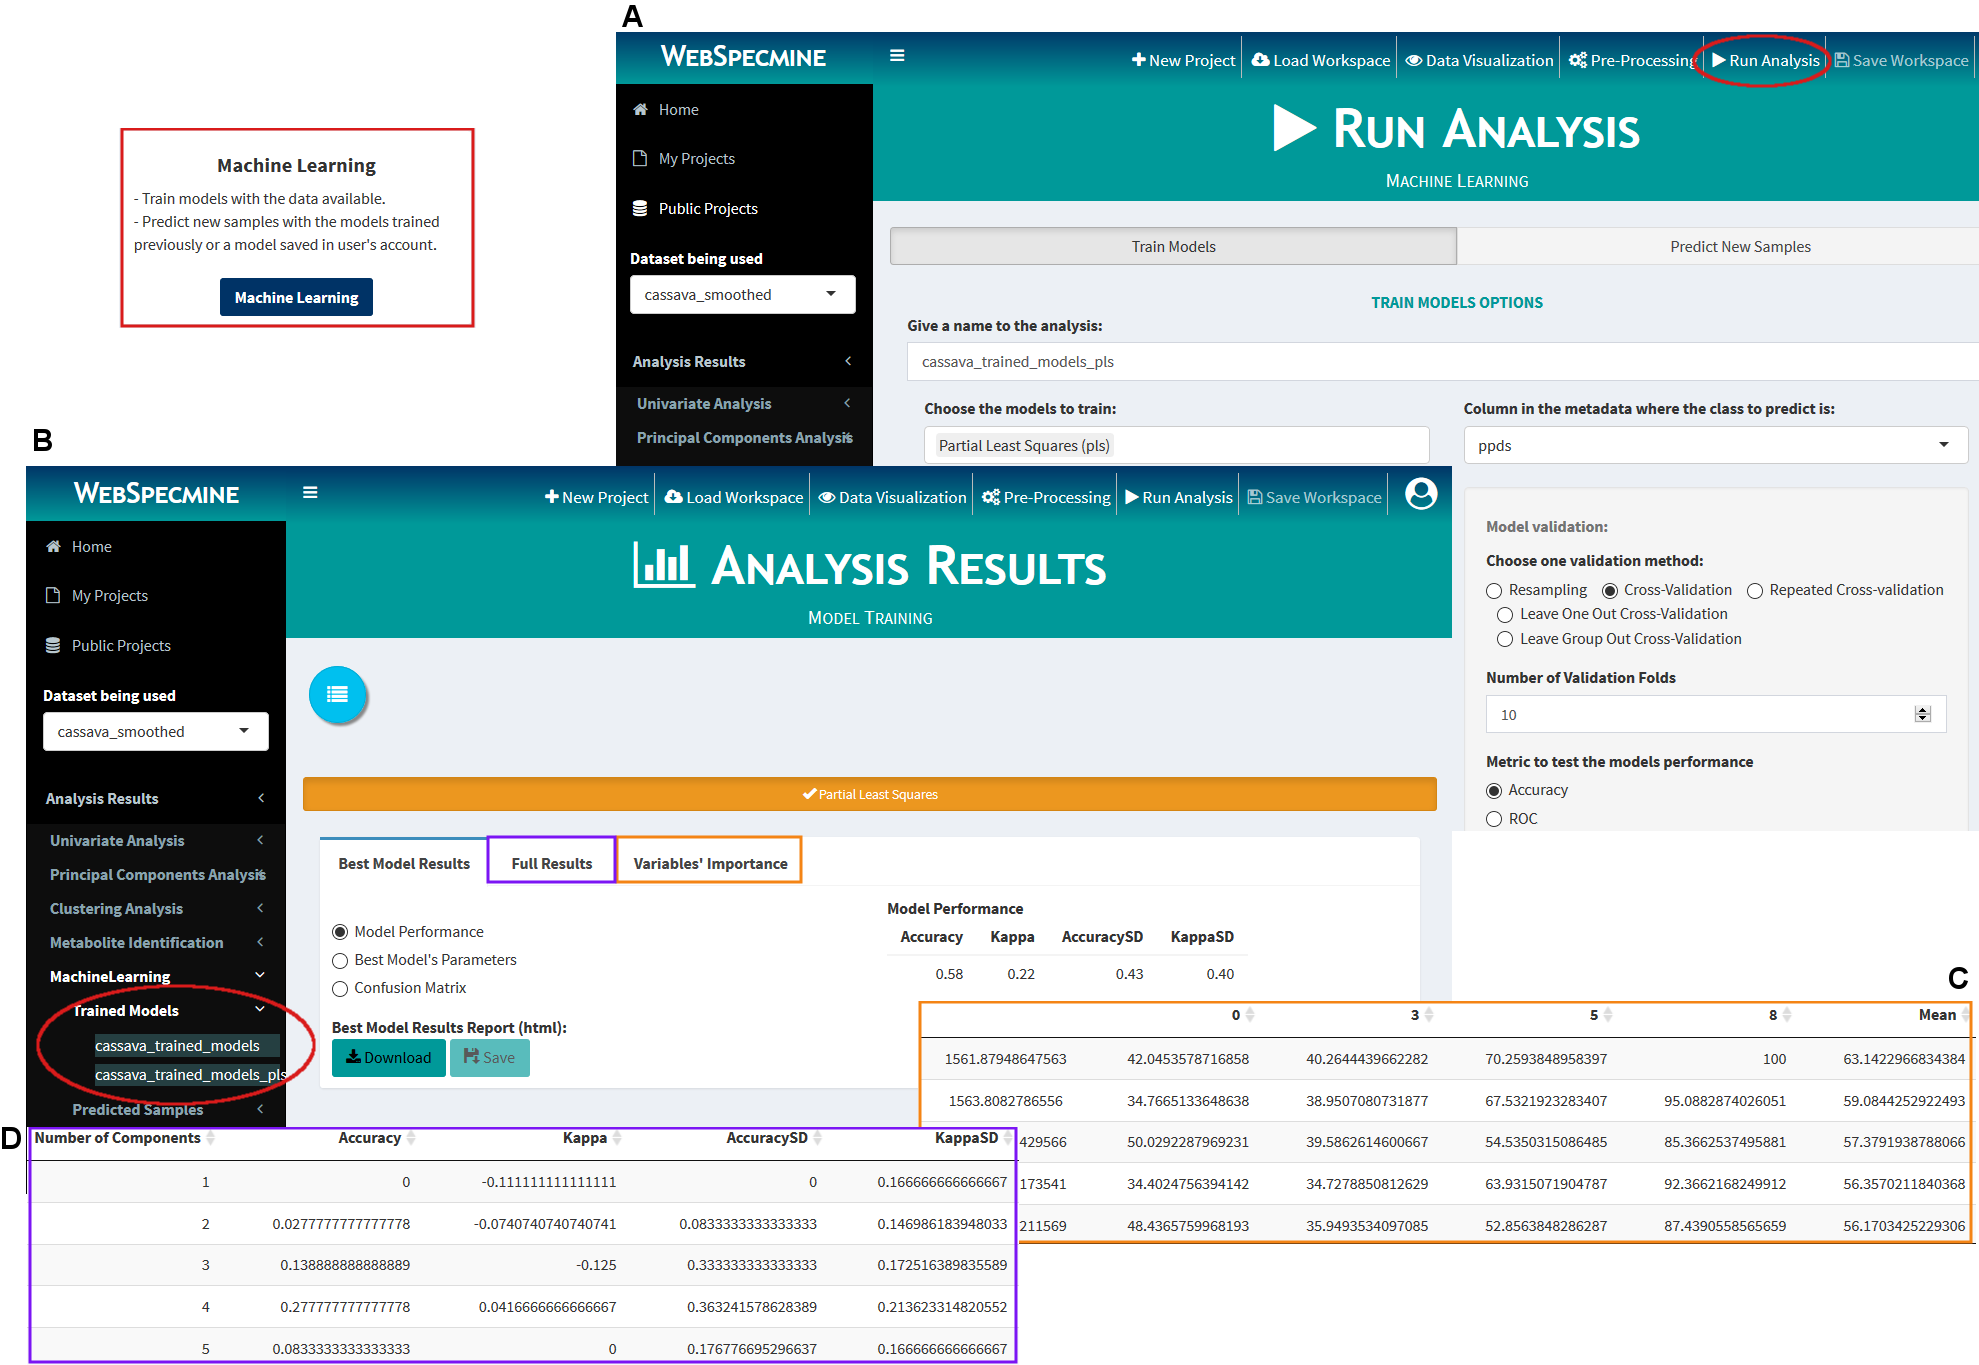
\includegraphics[width=1\linewidth]{Imagens/CassavaPPD/ml}
	\caption{\textit{Run Analysis} page for machine learning analysis (\textbf{A}) and respective results page showing the performance metrics for the \gls{pls} model (\textbf{B}), the full results from the tuning parameters for this model (\textbf{C}) and the variable importance table (\textbf{D}).}
	\label{cassava_machine_learning}
\end{figure}


The machine learning results show that the \gls{pls} model accurately predicted the samples' class about 58\% of the times, with the most relevant features for the classification being the wavenumbers around 1560 $cm^{-1}$.

The full analysis reports performed using the \textit{specmine} package for this study can be accessed at \href{http://darwin.di.uminho.pt/metabolomicspackage/cassava.html}{\nolinkurl{http://darwin.di.uminho.pt/metabolomicspackage/cassava.html}}.




